\newpage
\chapter*{Introduction}
\addcontentsline{toc}{chapter}{Introduction}
%This is typically an outline description detailing the background to the problem.

%
\newglossaryentry{DAM}
{
  name={DAM},
  description={decameter radio emissions in the 10-100 m wavelengths},
  sort=DAM
}
%

It was discovered in 1954 by \cite{burke55} that the planet Jupiter emits radio transmissions in the decameter (\gls{DAM}) range \textit{(10-100 m wavelengths)}, and the inner Jovian satellite Io appeared to have a strong control effect on these emissions \citep{belcher87}. Jupiter's radio emissions range between 4 MHz to 40 MHZ while emitting most strongly at 8 MHz  \citep{wilkinson94}. Due to interference from human short wave radio sources between 4-15 MHz coupled with the attenuation of these signals below 8 MHz or the refraction off Earth's ionosphere, the majority of emissions have been observed up in the 15-25 MHz range where this interference is less \citep{wilkinson94}. The emission signal strength quickly diminishes above this range for ground based listening sites \citep{wilkinson94}.

%
\begin{figure}[here]
\centering
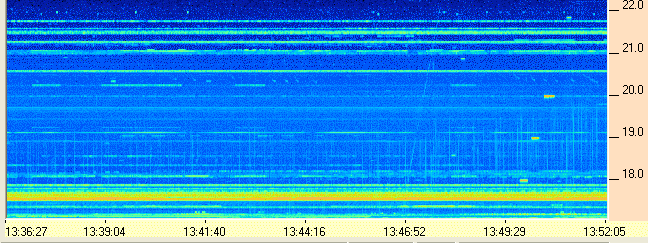
\includegraphics[width=8cm]{images/01}
\caption{Decametric Radio Emissions \citep{ashcraft13}}
\label{fig:dam_Emissions}
\end{figure}
%

Data collected by the two Voyager spacecraft in 1979 \citep{belcher87} and the later Galileo mission in 1995 \citep{kivelson96} added hugely to the understanding of the plasma interactions between Jupiter and Io and the source of the \gls{DAM} emissions. It was discovered that the Io has a thin atmosphere made up of a number of neutral gasses namely sodium, potassium, sulphur, and oxygen as shown in Figure.~\ref{fig:io_neutral_gasses} on page~\pageref{fig:io_neutral_gasses}. It is generally thought these gasses have been emitted through volcanic activity on the surface of the moon \citep{belcher87}. The gasses in orbit of Io have a very short life time, due to collisions with magnetospheric electrons. This gives rise to a plasma torus (\gls{IPT}) which co-rotates with Jupiter itself \citep{belcher87}. This can also be seen in Figure.~\ref{fig:io_neutral_gasses} on page~\pageref{fig:io_neutral_gasses} which shows the \gls{IPT}.

%
\begin{figure}[here]
\centering
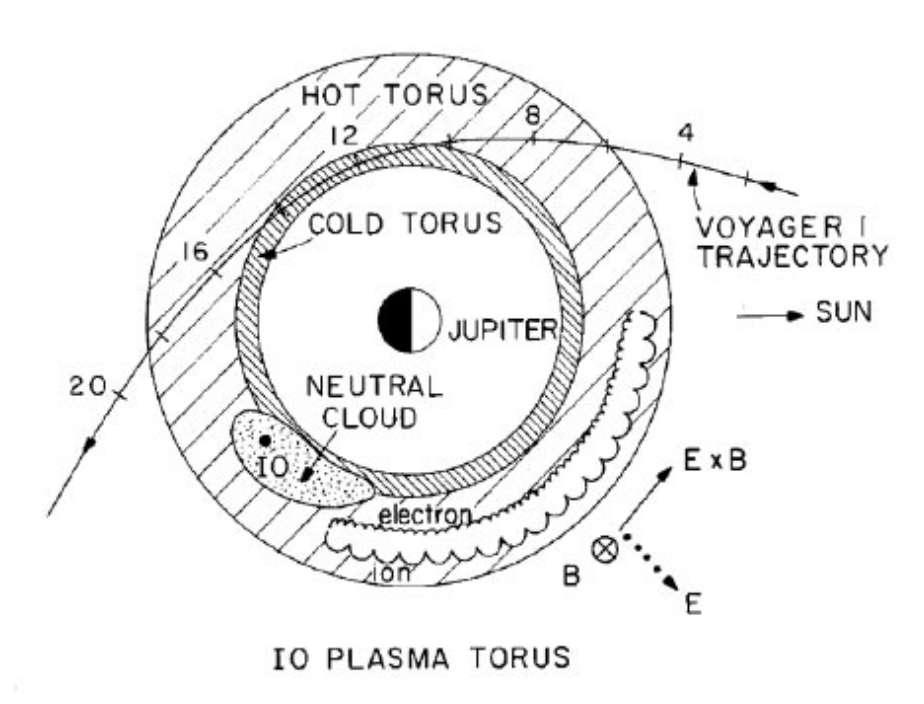
\includegraphics[width=8cm]{images/02}
\caption{Neutral Gasses in Orbit of Io \citep{belcher87}}
\label{fig:io_neutral_gasses}
\end{figure}
%

%
\newglossaryentry{IPT}
{
  name={IPT},
  description={Io Plasma Torus is created by Jovian atmospheric electrons ionizing neutral atmospheric gas such as sulphur in orbit around Io},
  sort=IPT
}
%

%
\newglossaryentry{IFT}
{
  name={IFT},
  description={Io Flux Tube is a cylindrical area of space containing magnetic field lines},
  sort=IFT
}
%

%
\begin{figure}[here]
\centering
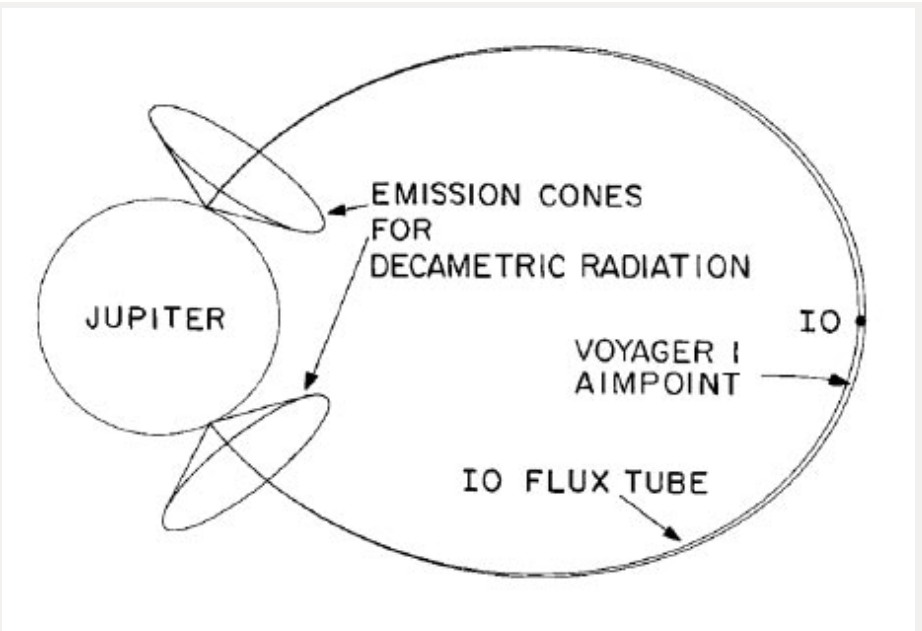
\includegraphics[width=6cm]{images/03}
\caption{Magnetic Flux Tube linking Jupiter and its satellite Io \citep{belcher87}}
\label{fig:io_flux_tube}
\end{figure}
%

The local co-rotation speed of the plasma torus is faster than the Keplerian orbit of the moon, and the plasma overtakes Io in its orbit at \begin{math} 57 km/s^{-1} \end{math} \citep{belcher87}. Figures.~\ref{fig:io_flux_tube}~and~\ref{fig:io_flux_tube_plasma_torus} on pages~\pageref{fig:io_flux_tube}~and~\pageref{fig:io_flux_tube_plasma_torus} detail diagrams of the Io Flux Tube (\gls{IFT}) which is a cylinder shaped tube of space containing Jovian magnetic field lines \citep{belcher87} which link Io to Jupiter's ionosphere at both poles. A large portion of the decametric emissions come from the area where this \gls{IFT} meets the Jovian ionosphere \citep{belcher87}. 

Io acts as a unipolar conductor as it orbits within this flux torus \citep{bose08}. Alfv\'en waves are regularly produced which carry an electric charge along the magnetic field lines between Io and Jupiter \citep{bose08} thereby acting as a standing wave \citep{bose08}. These Alfv\'en waves reflect between Jupiter's ionosphere at poles and Io up to 9 times \citep{bose08} before dissipating as they follow Io through its orbit. 

It appears the source of the \gls{DAM} emissions are largely due to these reflections of the Alfv\'en waves off Jupiter's ionosphere in both the northern and southern regions \citep{bose08}. See Figure.~\ref{fig:io_plasma_torus} on page~\pageref{fig:io_plasma_torus} which shows the Alfv\'en wings reflecting from Jupiter's Ionosphere creating emission cones.

The \gls{DAM} emissions radiate outwards in the shape of a cone as show in Figure.~\ref{fig:io_flux_tube} on page~\pageref{fig:io_flux_tube} \citep{belcher87}. When Io is at specific points in its orbit of Jupiter, these emission cones are pointing in the direction of Earth, at which point emissions can be picked up at ground based radio telescope listening stations.

%
\begin{figure}[here]
\centering
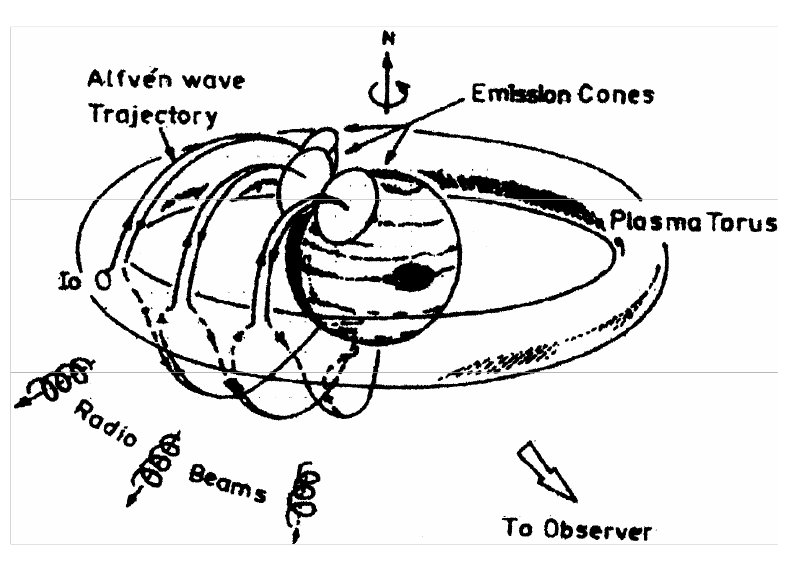
\includegraphics[width=8cm]{images/04}
\caption{Alfv\'en Waves following Io through its orbit and the DAM Emission cones \citep{bose08}}
\label{fig:io_plasma_torus}
\end{figure}
%

%
%%%%%%%%%%%%%%%%%%%%%%%%%%%%%%%%%%%%%%%%%%%%%%%%%%%%%%%%%%%%%%%%%%%%%%%%%%%%%%%%%%%%%%%%%%%
%
%\newpage
%\section*{Research Topic}
%\addcontentsline{toc}{section}{Research Topic}
%Students should identify whether the research outcomes are likely to have universal application or have a defined scope. This is important in gauging the extent to which the work is capable of independent replication.
%

%
\newglossaryentry{WRC}
{
  name={WRC},
  description={World Radio Communication Conference},
  sort=WRC
}
%

%
\newglossaryentry{HF}
{
  name={HF},
  description={High Frequency usually refers to radio frequencies in the 3 - 30 MHz},
  sort=HF
}
%

A ground based listening station aiming to record \gls{DAM} emissions from Jupiter is most likely to succeed between 15-25 MHz \citep{wilkinson94}. According to \cite{arrl-00} there is no clear definition of the \textit{shortwave} radio bands however it is most often considered to extend from 3 MHz to 30 MHz. ComReg is the Irish Commission for Communications Regulation within Ireland, and maintains a list of the short wave frequencies which are designated for transmission purposes in Ireland and can be seen in Figure.~\ref{fig:irish_electromagnetic_transmission_ranges} on page~\pageref{fig:irish_electromagnetic_transmission_ranges} \citep{comreg14}.

%
\begin{figure}[here]
\centering
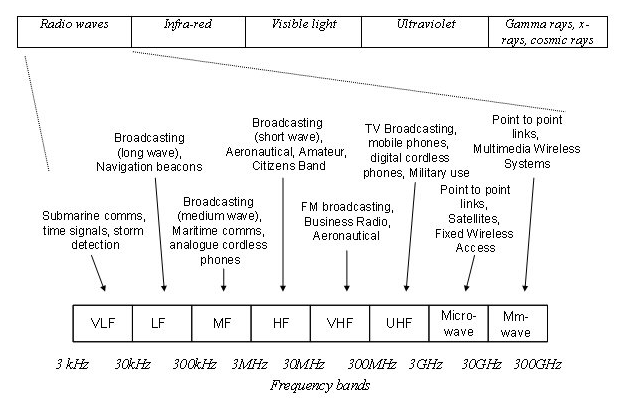
\includegraphics[width=8cm]{images/06}
\caption{Irish Regulatory Transmission Ranges \citep{comreg14}}
\label{fig:irish_electromagnetic_transmission_ranges}
\end{figure}
%

As many commercial short wave radio stations transmit in the lower end of the high frequency (\gls{HF}) 3-7 MHz range, it can be extremely busy and potentially difficult to monitor \gls{DAM} emissions where they are strongest. Amateur Radio operators also operate frequently in mid-late \gls{HF} ranges (\textit{160 m, 80 m, 60 m, 40 m, 30 m, 20 m, 17 m, 15 m, 12 m and 10 m bands}) while the higher frequency \gls{DAM} emissions taper off in strength very quickly. This limits the potential listening range significantly. Despite these obstacles, there are sections of the \gls{HF} spectrum which are suitable to capture Jovian emissions. One frequency to monitor Jovian \gls{DAM} emissions which is recommended by the Radio Jove project is \textit{20.1 MHz} \citep{nasa12}. 

Sourcing a suitable antenna is one of the first requirements to satisfy in order to capture \gls{DAM} emissions. Antennas are generally best suited to collect electromagnetic radiation at single specific frequencies, but may resonate and therefore operate over a range of frequencies depending on the design \citep{nasa12}. The wavelength ($\lambda$) which corresponds with the frequency (\textit{f}) \textit{20.1 MHz} can be obtained using the wavelength equation as shown in fig \ref{fig:wavelength_equation}. The corresponding wavelength for the frequency \textit{20.1 MHz} works out to be \textit{14.925 m} using this equation.

%
\begin{figure}[here]
  \centering
  \begin{equation}  	
    \lambda = \frac{c}{f}
  \end{equation}
  \begin{equation}
    \lambda = \frac{3\times10^8 m/s}{20.1\times10^6 Hz} = 14.925373134328359 m
  \end{equation}
  \caption{Wavelength Equation}
  \label{fig:wavelength_equation}
\end{figure}
%

One simple antenna design for collecting \gls{DAM} emissions is the \textit{dipole}. A dipole antenna can be constructed simply and cheaply from two pieces of wire and three insulators \citep{nasa12}, while ensuring to cut the wires to a length matching half the desired wavelength being captured \citep{nasa12}. However as the formula referenced in Figure.~\ref{fig:wavelength_equation} on page~\pageref{fig:wavelength_equation} describes the use of an \textit{infinitely thin} wire which is not possible in reality, \textit{capacitive end effects} must be taken into account when working out the resonating wavelength for a dipole antenna \citep{nasa12}.

The formula for calculating the resonating frequency for a half wavelength dipole is described in Figure.~\ref{fig:wavelength_equation_dipole} on page~\pageref{fig:wavelength_equation_dipole} and produces the value which should measure from tip to tip on the wires used to construct the dipole antenna \citep{nasa12}. \cite{RSGB-14} states in practice that the true resonance is not exactly multiples of the half-wavelength due to factors such as the coatings on the wire and loss due to radiation. A second formula is detailed in Figure.~\ref{fig:wavelength_equation_wire_antenna} on page~\pageref{fig:wavelength_equation_wire_antenna} which takes these factors into account and produces an antenna length which is slightly larger than the formula proposed by \citep{nasa12}. In Formula: 4 \textit{n} stands for the number of half-wavelengths in the antenna.

%
\begin{figure}[here]
  \centering
  \begin{equation}  	
    \bigg(\frac{\lambda}{2}\bigg)m = \frac{142.65}{20.1 MHz} = 7.097014925373134 m
  \end{equation}
  \caption{Wavelength Equation for Real World Half Wavelength Dipole Antenna}
  \label{fig:wavelength_equation_dipole}
\end{figure}
%

%
\begin{figure}[here]
  \centering
  \begin{equation}  	
    \lambda m = 155 \bigg(\frac{n - 0.05}{f}\bigg)
  \end{equation}
  \begin{equation}  	
    \lambda m = 155 \bigg(\frac{1 - 0.05}{20.1 MHz}\bigg)  = 7.325870646766169 m
  \end{equation}
  \caption{Wavelength Equation for Real World Half Wavelength Wire Antenna}
  \label{fig:wavelength_equation_wire_antenna}
\end{figure}
%

The radio emissions come in several different forms each with slightly different characteristics. Table. \ref{tab:dam_emissions} shows a list of the more widely known types which can be picked up using ground based listening equipment, and also has some information about their different characteristics \citep{wilkinson94}. Any particular observation session might be made up of some or all of these different types of \gls{DAM} emission and can last from a few minutes to several hours for larger noise storms \citep{wilkinson94}.

%
\begin{table}
  \centering
  \begin{tabular}[pos]{| c | c | c |}
    \hline
    Type & Emission Length & Emission Description\\ \hline
    S-Bursts & short generally 1-10 milliseconds & wideband bursts, several MHz wide\\ \hline
    L-Bursts & long 0.5 - 5 seconds & wideband bursts, several MHz wide\\ \hline
    N-Bursts & milliseconds upto seconds & narrowband bursts, several kHz wide\\
    \hline
  \end{tabular}
  \caption{Most common types of DAM Emissions from Jupiter \citep{wilkinson94}}
  \label{tab:dam_emissions}
\end{table}
%

Figure.~\ref{fig:dam_emissions_spectrum} on page~\pageref{fig:dam_emissions_spectrum} shows an ideal case of the \textit{S-Burst} and \textit{L-Burst} \gls{DAM} emissions and what they might look like on a frequency spectrum graph. S-Burst emissions are short, generally 1-10$\times10^{-3}s$ long while L-Bursts can often be between 0.5-5s in length.

%
\begin{figure}[here]
\centering
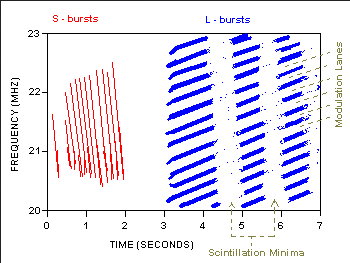
\includegraphics[width=8cm]{images/05}
\caption{Ideal DAM Emissions types from Jupiter \citep{wilkinson94}}
\label{fig:dam_emissions_spectrum}
\end{figure}
%

%%%%%%%%%%%%%%%%%%%%%%%%%%%%%%%%%%%%%%%%%%%%%%%%%%%%%%%%%%%%%%%%%%%%%%%%%%%%%%%%%%%%%%%%%%%
%
\newpage
\section*{Research Hypothesis}
\addcontentsline{toc}{section}{Research Hypothesis}
%
\newglossaryentry{SDR}
{
  name={SDR},
  description={Software Defined Radio is the creation of radio functions within software rather than hardware},
  sort=SDR
}

The aim of this project is to design and construct a low cost, self sufficient software defined radio (\gls{SDR}) telescope listening station, which can capture signals for transmission to a central data aggregation point for signal processing and analysis. This telescope should be suitable to study signals  in the \gls{DAM} (10-100 m) band at or near the \textit{20.1 MHz} frequency in order to pick up emissions produced by either Jupiter or the Sun.

There are a number of challenges which need to be overcome to achieve this, such as Jupiter only being visible for a number of months each year and then generally in the evening, night, or morning hours. Often at highly unsociable times. For this reason a radio telescope listening site should be as automated as possible.

%
\begin{figure}[here]
\centering
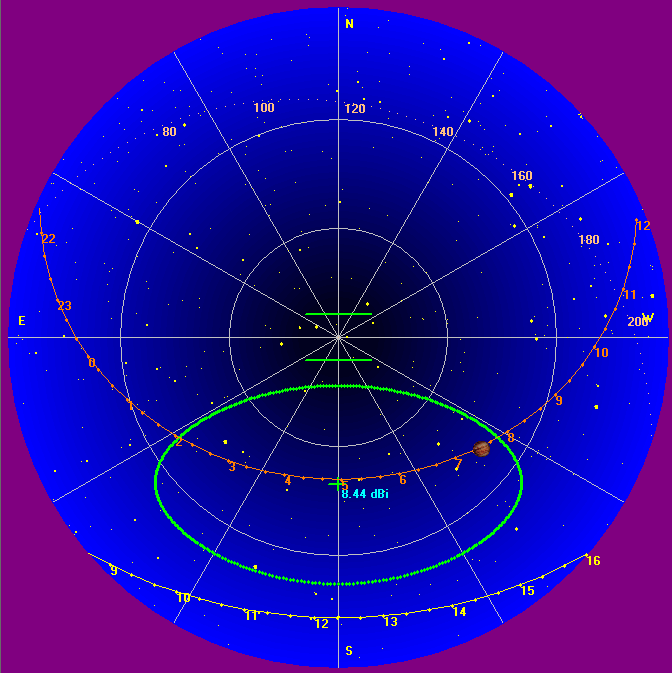
\includegraphics[width=8cm]{images/07}
\caption{Dual Dipole Antenna Beam at 20FT and 135deg phasing South \citep{nasa12}}
\label{fig:dual_dipole_20ft_135phasing_s}
\end{figure}
%

During daylight hours, the ionosphere becomes opaque to signals in the \gls{DAM} band due to becoming ionised by solar radiation \citep{nasa-ionosphere-12}. The proposed system will have a short window in the order of 1-6 hours every second night and early morning. During which it may be possible to capture \gls{DAM} emissions from Jupiter. The Sun is a source of \gls{DAM} emissions also, and the telescope can capture solar storm emissions without modification, providing the Sun passes through the antenna beam. The telescope may require manual reconfiguration in order to pick up solar storm emissions during the day.


%
\begin{figure}	
	\centering
	\begin{subfigure}[t]{5cm}
		\centering
		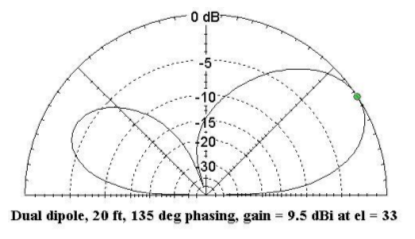
\includegraphics[width=5cm]{images/09}
		\caption{Dual Dipole Antenna Array Beam \citep{nasa12}}
		\label{fig:dual_dipole_antenna_array_beam}	
	\end{subfigure}
	\quad
	\begin{subfigure}[t]{5cm}
		\centering
		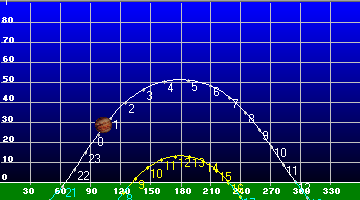
\includegraphics[width=5cm]{images/11}
		\caption{Radio Jove graph showing Jupiter's max altitude 2014 \citep{rjp-14}}
		\label{fig:jupiter_max_altitude_2014}
	\end{subfigure}
	\caption{Dipole antenna characteristics and Jupiter's altitude}
	\label{fig:dipole_beam_jupiter_altitude}
\end{figure}
%

Interference from human sources such as short wave radio stations or amateur radio operators are also likely to affect the collection of \gls{DAM} emissions from Jupiter. The ability for automated flagging or removal of interference would be a desirable feature of the system. Lightning storms can also produce interference which will affect observations, it might be desirable for the system to handle natural interference sources also.

%
\begin{figure}[here]
\centering
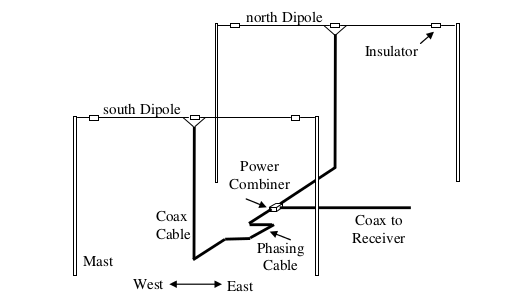
\includegraphics[width=8cm]{images/08}
\caption{Dual Dipole Antenna Array \citep{nasa12}}
\label{fig:dual_dipole_antenna_array}
\end{figure}
%

%This should outline the approach and methodology being proposed by the student to address the research question.
\newpage
\section*{Methodology}
\addcontentsline{toc}{section}{Methodology}
The section aims to provide a summary of the methodologies which will be followed on this project in order to answer the research questions put forward in the next section. It is broke up into the following subsections:

\begin{description}
  \item[Antenna Build] \hfill \\
    Building the antenna is further broken down into the following steps:
    \begin{itemize}
      \item source materials to build a dual dipole antenna
      \item build the telescope antenna
      \item validate the antenna is capable of collecting signals at or near the 20.1 MHz frequency \\
    \end{itemize}
  \item [Analysis of Listening Site Suitability] \hfill \\
    Finding a site suitable to deploy the antenna will require a site survey with the antenna connected to a spectrum analyser. The spectrum analyser can be used to visualise many hours of averaged data and estimate the frequencies which are most active at this site.
    \begin{itemize}
      \item source a spectrum analyser suitable for performing a site survey
      \item perform the survey at this site
      \item repeat until suitable site is found 
      \item deploy the antenna at a site \\
    \end{itemize}
  \item [Data Collection] \hfill \\
    Jupiter is visible above the horizon at night only during certain periods see Figure.~\ref{fig:dual_dipole_antenna_array_beam} on page~\pageref{fig:dual_dipole_antenna_array_beam}. In order to perform the required data collection it is highly desirable to automate the process if possible.
    \begin{itemize}
      \item create listening schedule during which \gls{DAM} emissions are likely to occur using the Radio Jove software
      \item develop \gls{SDR} prototype mechanism for gathering raw data from the antenna\\
    \end{itemize}
  \item [Data Analysis] \hfill \\
    Collected data can be analysed manually at first in order to validate the testbed, but later using software such as the development of basic algorithms to spot events such as \textit{S-Bursts} occurring in the data.
    \begin{itemize}
      \item analyse data collected for evidence of Jovian or Solar \gls{DAM} emissions
      \item analyse data for evidence of interference from human sources
      \item analyse data for evidence of interference from natural sources
      \item develop a system which connects to the worldwide dxcluster system and creates flag events for human identified emissions at or near the target frequency being monitored by the telescope
      \item develop a system which interacts with the Blitzortung servers and creates flag events for emissions generated by lightning \\
    \end{itemize}
  \item [Design Platform] \hfill \\
    An analysis of the current available \gls{IOT} technologies and some of the available options which could be used in order to produce an open low cost platform which amateur astronomers could use in order to study emissions in the \gls{DAM} band.
    \begin{itemize}
      \item design a low cost platform suitable for collection of signals to produce power plots or spectrograms in order to identify \gls{DAM} emissions originating from Jupiter\\
    \end{itemize}
\end{description}


The \gls{SDR} hardware transceiver used is likely to be the \textit{HackRF} system while the \gls{SDR} software components will be developed in either \textit{C++} or \textit{Python} as both languages have bindings for the \textit{GNURadio} development tool-kit \citep{gnuradio-14}. The backend aggregation system with API will most likely be developed in the \textit{Ruby} language as this language is highly expressive and suitable for rapid prototype development. Execution of the Ruby application on the Java VM is capable using the \textit{JRuby} system, which will also allow the incorporation of any required Java libraries.

%
%%%%%%%%%%%%%%%%%%%%%%%%%%%%%%%%%%%%%%%%%%%%%%%%%%%%%%%%%%%%%%%%%%%%%%%%%%%%%%%%%%%%%%%%%%%
%
\newpage
\section*{Research Questions}
\addcontentsline{toc}{section}{Research Questions}
%A clear, precise definition of the problem is very important to focus on the research activity. great care should be used in devising the research questions. They define the structure of the investigation/innovation that will be used and an essential metric of the quality of the dissertation is the degree to which the research question has/have been answered.
The initial research questions which arise are as follows:

%
\newglossaryentry{IOT}
{
  name={IOT},
  description={Internet of Things a buzzword for everything connecting to everything},
  sort=IOT
}

\newglossaryentry{IQ}
{
  name={IQ},
  description={Imaginary Quadrature signal - Complex signal data and quadrature phase values in a digital signal sample},
  sort=IQ
}
%

\begin{enumerate}
  \item \textit{What current Internet of Things (\gls{IOT}) technologies would best suit the development of a software defined radio signal listening station and how cheaply can it be created?}
  \begin{itemize}
  	\item How expensive would a renewable power supply solution such as solar be?
  	\item Can a low powered computing platform such as the Raspberry Pi B+ suitably host the system, or will a more powerful platform be required?
  	\item How feasible are wireless technologies such as Zigbee, WIFI or Bluetooth to stream collected data to a central facility?
  \end{itemize}
  
  \item \textit{What processes or algorithms need to be developed to filter or flag known instances of human interference from radio signal observations?}
  \begin{itemize}
  	\item Flag transmission signals identified by amateur radio enthusiasts from a local DXSpider server in recorded data.
  	\item Flag instances of natural radio interference such as lightning from the Blitzortung server in recorded data.
  \end{itemize}
  
  \item \textit{What \gls{SDR} tools, processes and or algorithms need to be developed to identify instances of the three main \gls{DAM} emission types detailed in Table. \ref{tab:dam_emissions}?}
  \begin{itemize}
  	\item Can existing tools and signal processing techniques be employed to find \gls{DAM} emissions?
  	\item What is required from an algorithm which might identify \gls{DAM} emissions within an \gls{IQ} signal?
  \end{itemize}
  
\end{enumerate}

%
%%%%%%%%%%%%%%%%%%%%%%%%%%%%%%%%%%%%%%%%%%%%%%%%%%%%%%%%%%%%%%%%%%%%%%%%%%%%%%%%%%%%%%%%%%%
%
\newpage
\section*{Literature Review}
\addcontentsline{toc}{section}{Literature Review}
%This should contain a review of a number of books, journal articles and web references of relevance to the research area proposed. The literature should contain seminal and recent referenced research material that is categorised under a number of relevant sub-themes.

The literature review can be broken down into the following areas:


\begin{itemize}
  \item[\textbullet] What are the decametric radio emissions and what are they caused by
  \item[\textbullet] Potential radio telescope designs which could be replicated in order to collect DAM emissions
  \item[\textbullet] Digital signal processing
\end{itemize}

\subsection*{Decametric Radio Emission what are they and where do they come from?}
\cite{belcher87} states that the data collected by both \textit{Voyager} spacecraft fit with the Alfv\'en wing theory as an explanation for the source of the \gls{DAM} emissions \citep{belcher87}. \cite{kivelson96} discusses the refinements made to this theory to take into account the flowing plasma between Jupiter's ionosphere and the electrically conducting Io. The \textit{Galileo} spacecraft collected data which appears to corroborate the updates to the Alfv\'en wing model \citep{kivelson96}. \cite{bose08} states that the Alfv\'en waves reflect off Jupiter's ionosphere which cause the \gls{DAM} emissions to radiate out from the point in Jupiter's ionosphere where it meets the \gls{IFT} in a cone shape. \cite{imai-08} proposes an update to this model to take into account the decade long shifts in \gls{DAM} emission patterns, and proposes an extension to the emission cone model to include a \textit{searchlight} shaped emission zone \citep{imai-08} see Figure.~\ref{fig:decametric_emissions_searchlight} on page~\pageref{fig:decametric_emissions_searchlight}.

\subsection*{Radio Telescope Designs, Which to Choose?}
The NASA project \textit{Radio Jove} recommended the dual dipole array design for a cheap low cost listening site as shown in Figure.~\ref{fig:dual_dipole_antenna_array} on page~\pageref{fig:dual_dipole_antenna_array} \citep{nasa12}. But it is by no means the only antenna design which would be capable of picking up the \gls{DAM} emissions. \cite{wilkinson94} recommends a slightly more advanced design, the \textit{folded dipole} which maximises the bandwidth available to the antenna \citep{wilkinson94}. \cite{greef-12} details a third alternative for collecting \gls{DAM} emissions, a shortwave loop antenna as can be seen in Figures.~\ref{fig:loop_antenna_design_a}, \ref{fig:loop_antenna_design_b} and \ref{fig:loop_antenna_design_c} on page~\pageref{fig:loop_antenna_design_a}.

\subsection*{Digital Signal Processing}
\cite{smith-03-a} explains that digital signal processing is a term used to describe the mathematics, algorithms and techniques used to manipulate signals after they have been converted from analogue to digital. \cite{freidt-13} holds that digital signal processing is the preferred means to process signals, for reasons such as stability and for its resistance to long term ageing effects that analogue systems suffer from. However as \cite{smith-03-b} points out, due to the nature of the conversion from analogue to digital, information is lost in this process. \cite{smith-03-b} maintains that the proper sampling of an analogue signal occurred if you can reconstruct the signal from the digital samples collected, and incorrect sampling will lead to loss of the original signal due to aliasing.

%
\begin{figure}[here]
\centering
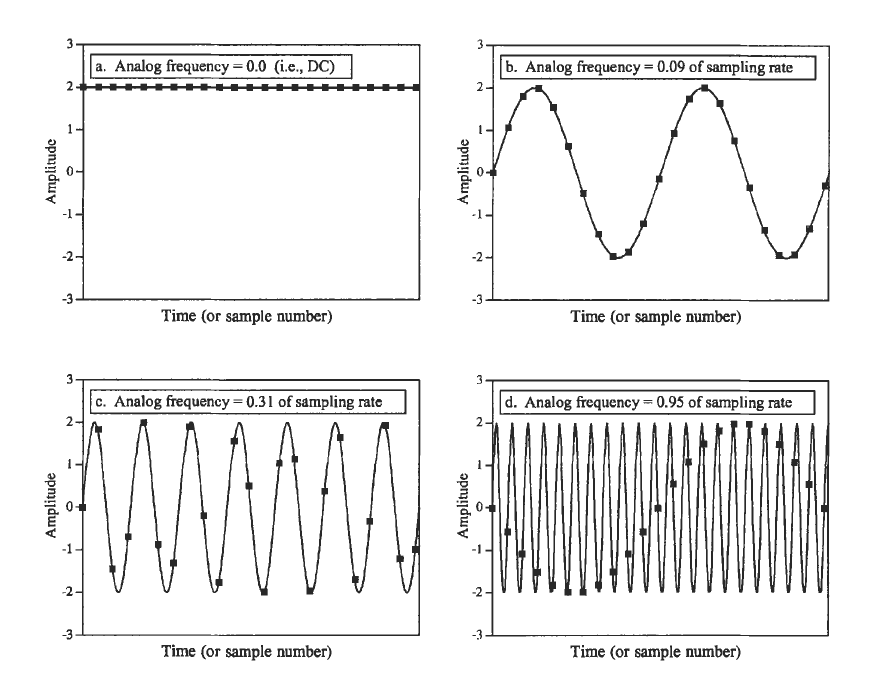
\includegraphics[width=8cm]{images/44}
\caption{Sampling an Analogue Signal \citep{smith-03-b}}
\label{fig:smith_sample_theorem_2003}
\end{figure}
%

\cite{smith-03-b} demonstrates in Figure.~\ref{fig:smith_sample_theorem_2003} on page~\pageref{fig:smith_sample_theorem_2003} how signal data loss occurs due to aliasing. When sampling an analogue signal which has a frequency more than half of the sample rate (Nyquist frequency), \cite{smith-03-b} observes that the original signal cannot be reconstructed. This is referred to as the sampling theorem \citep{smith-03-b} where $f_s$ is the sample rate and $f$ is the frequency being sampled.

%
\begin{figure}[here]
  \centering
  \begin{equation}  	
    f_s > 2f
  \end{equation}
  \caption{Sampling Theorem aka Nyquist-Shannon sampling theorem \citep{smith-03-b}}
  \label{fig:nyquist-shannon-sample-theorem}
\end{figure}
%

\cite{ossmann-15-b} contends that the application of Nyquist-Shannon sampling theorem only applies to real analogue signals where the bandwidth is equal to half the sample rate. However for a complex digital signal  the bandwidth is equal to the sample rate \citep{ossmann-15-b}.

Due to the cheap availability of computational resources, digital signal processing is capable of being carried out now within software entirely, this has led to the development of software defined radio solutions \citep{freidt-13}. The GNURadio software allows creation of software defined radio solutions by replacing hardware functions with modular software functions. These software functions are capable of being connected together, an output from one function providing input for another. It is in this fashion it is possible to transform digital signals using digital signal processing methods within the GNURadio platform\citep{gnuradio-14}.

%
\begin{figure}[here]
\centering
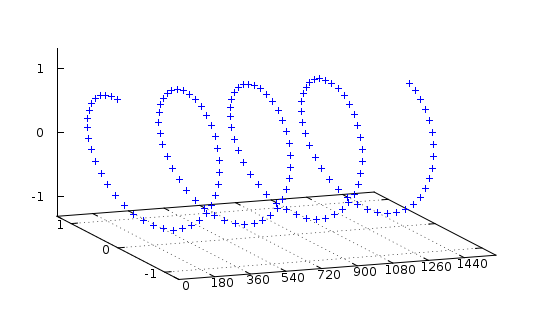
\includegraphics[width=7cm]{images/48}
\caption{I/Q Samples Helix \citep{kuisma-14}}
\label{fig:kuisma-iq-helix}
\end{figure}
%

\cite{ossmann-15-a} illustrates how the HackRF One \gls{SDR} transceiver can be accessed within GNURadio by way of the osmocomm source which is an abstraction layer between GNURadio and the HackRF driver. Figure.~\ref{fig:ossmann_am_demodulation} on page~\pageref{fig:ossmann_am_demodulation} shows an amplitude modulation signal which has been digitally sampled. In order to demodulate such a signal, an understanding how the signal data is stored is a must. Digital periodic signal samples tend to be stored in a complex format which amounts to polar coordinates \citep{ossmann-15-c}. $I$ is the point on the real axis, and $Q$ is an angle which contains the imaginary component. See Figure.~\ref{fig:kuisma-iq-helix} on page~\pageref{fig:kuisma-iq-helix} shows how these I/Q values are plotted periodically and Figure.~\ref{fig:kuisma-iq-polar} on page~\pageref{fig:kuisma-iq-polar} shows the I/Q polar data \cite{kuisma-14}.

%
\begin{figure}[here]
	\centering
	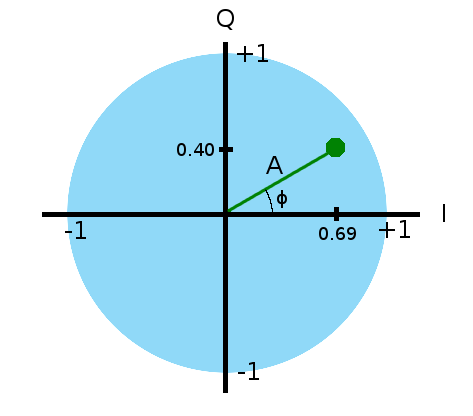
\includegraphics[width=8cm]{images/47}
	\caption{I/Q Samples Polar Plot \citep{kuisma-14}}
	\label{fig:kuisma-iq-polar}
\end{figure}
%

%
\begin{table}
  \centering
  \begin{tabular}{ | p{2.5cm} || p{2.5cm} | p{2.5cm} | p{2.5cm} | p{2.5cm} |}
    \hline
    \textbf{Topic} & \textbf{Belcher 1987} & \textbf{Kivelson et al 1996} & \textbf{Bose et al 2008} & \textbf{Imai et al 2008} \\ \hline \hline
    What are the Jovian DAM emissions and what causes them? & Large fraction of DAM emissions come from point where IFT meets Jupiter's ionosphere (p3). Large moving conductor within a magnetised plasma (p1) produces Alfv\'en wing. & Alfv\'enic disturbances, generated by flowing plasma from Jovian magnetosphere and conducting Io (p337). & Alfv\'en waves reflecting off Jupiter's Ionosphere (p79). & Not fully understood, but believed to be produced by cyclotron maser instability \citep{imai-08}. \\ \hline \hline

    \textbf{Topic} & \textbf{Wilkinson et al 1994} & \textbf{NASA Radio Jove 2012} & \textbf{Greef 2012} &  \\ \hline \hline

    Radio telescope designs suitable to capture DAM emissions from Jupiter & Wilkinson et al suggest a folded dipole antenna design & Radio Jove project suggest a dual dipole antenna & Greef demonstrates a low cost Loop Antenna design with reflection plate & \\ \hline \hline
    
    \textbf{Topic} & \textbf{Smith 2003} & \textbf{Freidt 2013} & \textbf{GNU Radio 2014} & \textbf{Ossmann 2015} \\ \hline \hline    
    
    Digital signal processing & Smith argues digital signal processing is one of the most powerful technologies that will shape the 21st century. & Freidt states digital signal processing now ubiquitous, and cheap availability of computational power lends self to software defined radio solutions. & GNURadio allows digital signal processing using transformation functions developed in software. & Ossmann argues that the HackRF One is perfectly suited as a low cost wide range transceiver for use within software defined radio prototypes. \\
    \hline
  \end{tabular}
  \caption{Literature Review Synthesis Matrix}
  \label{tab:literature_review_synthesis_matrix}
\end{table}
%